%!TEX root = p.tex
\section{Entity 1.1}

\begin{figure}[htb]
  \centerline{
    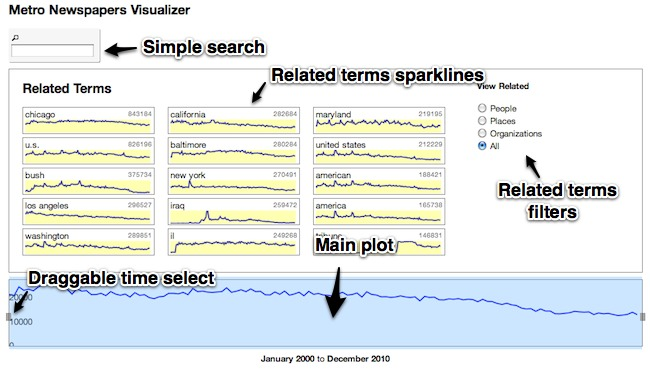
\includegraphics[scale=0.28]{figures/relation-0.jpg}
  }
  \caption{TODO: FILL ME IN}
  \label{fig:explorer-0}
\end{figure}

The first iteration of the entity relation viewer was designed to allow the user to quickly navigate between terms and entities related to a base query. Similar to how a user of wikipedia will follow links between related articles and discover new material, users of the entity relation viewer can quickly jump from topic to topic in search of a hidden story buried in the data.

\section{Entity 1.2}


\begin{figure}[htb]
  \centerline{
    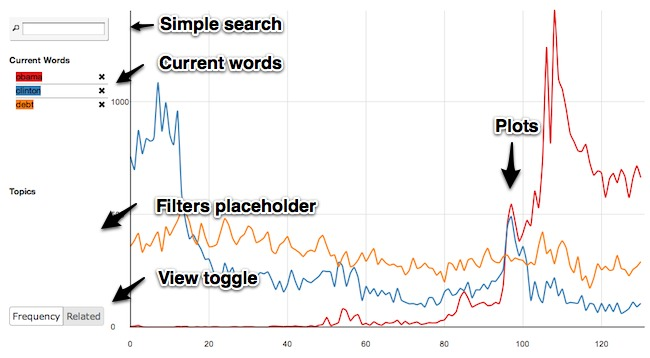
\includegraphics[scale=0.28]{figures/relation-1-a.jpg}
  }
  \caption{TODO: FILL ME IN}
  \label{fig:explorer-1-a}
\end{figure}

The second version of the entity relation viewer prototype was designed with many of the design decisions as the first version. Again quick exploration of related terms and a simple query  methodology were the heart of the design. This prototype does differ from the first version in one major way. In particular it allows frequency comparisons between different terms and assumes this will be at least as useful of an exploration method. As such it give people two way to explore terms; one for related terms and one for frequency comparisons.


\begin{figure}[htb]
  \centerline{
    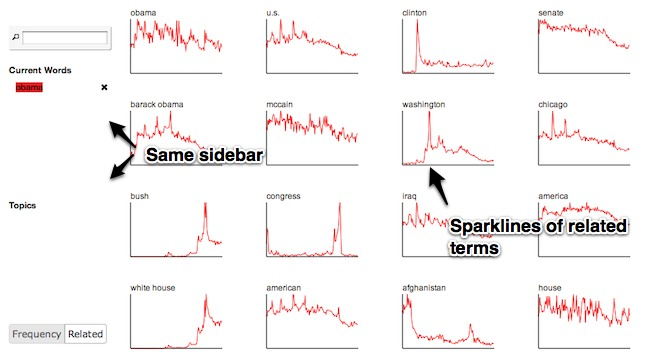
\includegraphics[scale=0.28]{figures/relation-1-b.jpg}
  }
  \caption{TODO: FILL ME IN}
  \label{fig:explorer-1-b}
\end{figure}
